\documentclass{atistandalonetask}
\usepackage{atistandard}
\begin{document}
  \begin{atiTask}[
    title = Heaviside-Funktion und Delta-Distribution
  ]
\begin{atiSubtasks}
\item Ein unendlich ausgedehntes, zweidimensionales Blatt mit Flächenmassendichte $\sigma_0$ werde durch die Flächengleichung $y=x^3$ beschrieben. Bestimmen Sie die Volumenmassendichte $\mu(x,y,z)$ dieses Blattes. 

\item Stellen Sie die in der Abbildung gegebene Funktion $g(x)$ mit Hilfe von \textsc{Heaviside}schen Sprungfunktionen dar (ohne Benutzung stückweiser Definitionen).  
  \begin{figure}[H]
\centering
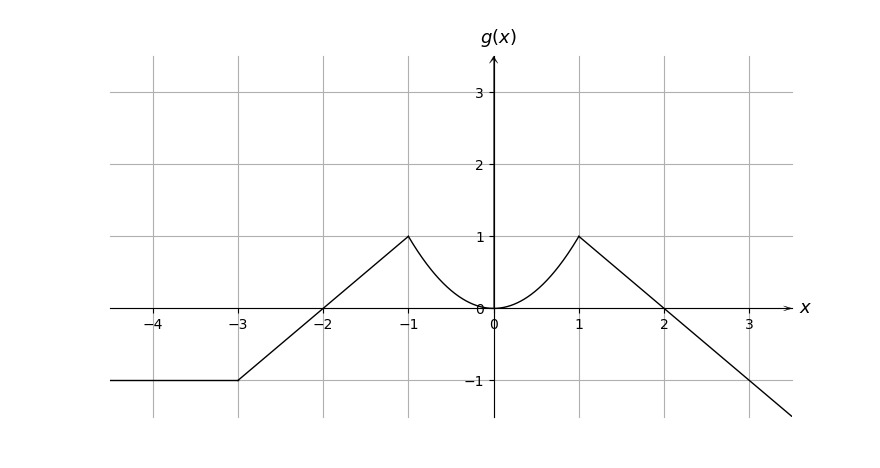
\includegraphics[width=0.8\linewidth]{./picture-heaviside_iib}
%\caption{durch Heaviside-Funktionen darzustellende Funktion}

\end{figure}
\end{atiSubtasks}
  	
  \end{atiTask}
  \begin{atiSolution}
   	Lösung folgt
  	%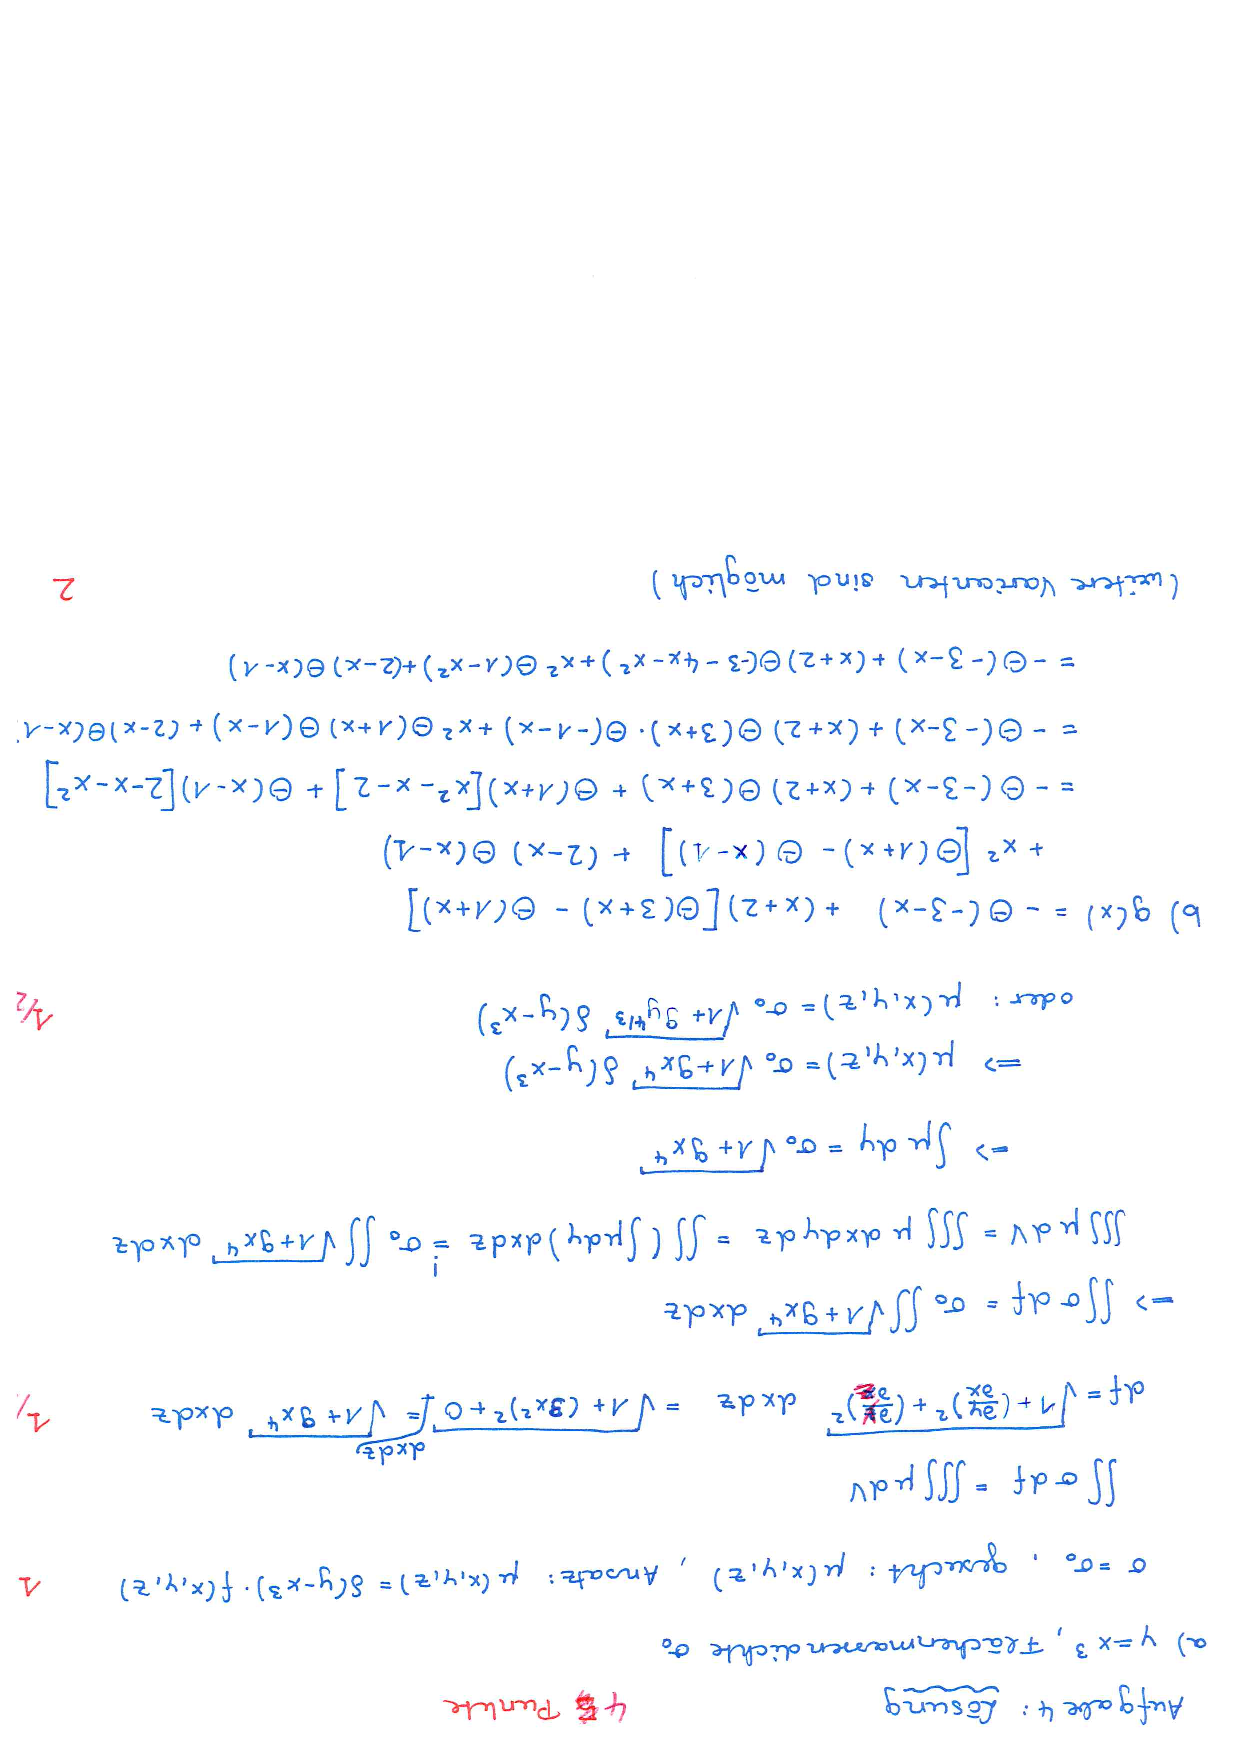
\includepdf[pages=-]{solution-heaviside_ii.pdf}
  \end{atiSolution}
\end{document}